\documentclass[12pt]{article}
\usepackage{3Rdefs}
\usepackage{graphicx}

\title{\iR{} Scientific Modelling}
\author{Ed Darnell}
\date{\today}

\begin{document}
\maketitle
\begin{abstract}
    This document clearly defines logic, \(\qbit\) and \iR{} scientific modelling. While our brains are proficient at creating \texttt{3D} models of the macroscopic world, they have inherent limitations. In everyday life, we often use oversimplified categories—right or wrong, true or false, 1 or 0—without fully understanding how logic is defined.

    \iR{} defines and explains, providing a consistent, relativistic understanding of reality and uncertainty. \iR{} has practical applications, from refining scientific inquiry to reshaping societal structures. By adopting an analytic approach to understanding reality, we empower ourselves to make more informed, ethical decisions that reflect the intricacies of our world.

    The aim here is not to discard traditional knowledge but to refine and correct it, opening up new avenues for progress and understanding. \iR{} enables a transition to relativistic modelling, the natural progression from powerful but sometimes illogical AI. It is essential we make this transition as quickly as practical. The future of our society, our species and our ecosystem depends upon it.
\end{abstract}
\section*{Logic, Models, and Reality}
To understand the cosmos, we must acknowledge a crucial fact: our perception of reality is filtered through mental models shaped by evolution for pragmatic survival, not for the objective dissection of the universe's fabric. These models, while sophisticated, are rooted in an evolutionary timeline that places Homo sapiens' cognitive leap merely 200,000 years ago. They are heavily influenced by survival imperatives that predate technology and complex social interaction.

While these neural constructs help us interact with our environment, they do not provide a direct view into the universe's functioning. Electromagnetic waves, gravity, and the quantum realm, for instance, are aspects of reality our ancestors never perceived; instead, they are elements we have come to model scientifically as our understanding of the universe has deepened.

In logic, \texttt{true} and \texttt{false} are defined within a logical framework. These are not inherent properties of reality but are definitions of the logical system. Binary logic, which first defines \texttt{0} as \texttt{NOT 1}, is foundational. This approach prevents ambiguity by providing a clear, base definition from which all subsequent definitions are consistently constructed. Logic is best viewed as a language, the language of mathematics and computing. In contrast to historic languages it is constructed in a way which prevents ambiguity or inconsistency.

Reality does not possess a \texttt{false} form and is provably not constructed from \texttt{0} and \texttt{1}. It exists independent of words, descriptions, logic and models. Reality is best modelled as continuous-relativity, whilst recognising any model will always lack some detail. Binary logic forms the best possible language to model reality. Words are neural, pre-logic language and whilst extremely important for non-scientific communication, should be viewed as scientifically ambiguous until defined within a logical model.

Logical models can both over-simplify and over-complicate. For example, with 100 random coin tosses, modelled as \( X \sim B(100,0.5) \), the model predicts a 99.99...\% chance of between 60 and 80 heads. The model cannot however predict the outcome of each individual toss, nor can it prevent all 100 coins being placed heads up (despite this outcome having a probability of less than  \( 8 \times 10^{-31} \)).

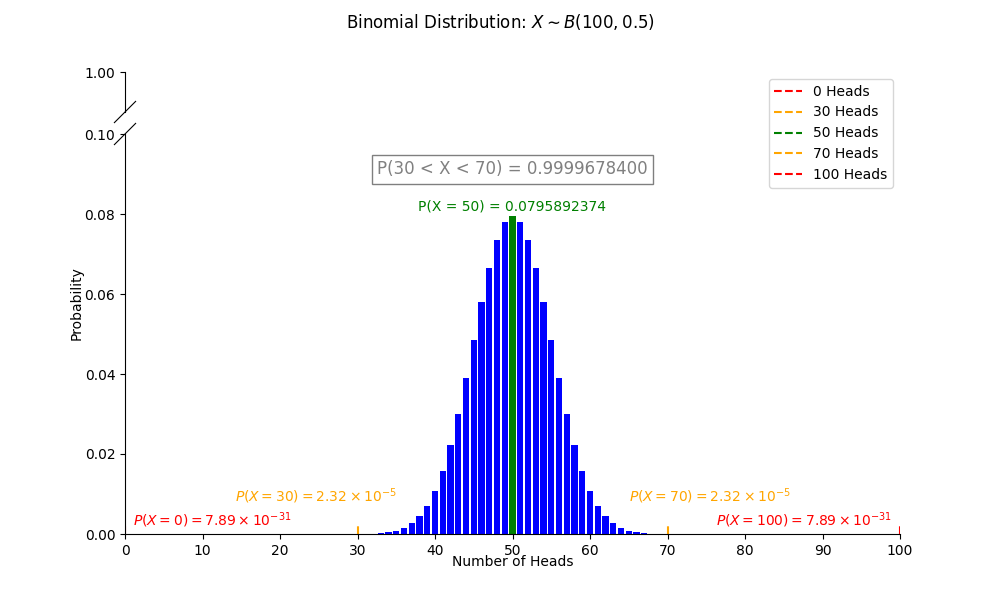
\includegraphics[width=0.95\textwidth]{binomial.png}

The logical model of coin tossing has a high degree of confidence if the assumption of randomness is met, but it is a model of reality, not reality. Logic can prove that no real event can be either perfectly random or perfectly causal. Models are always uncertain and science must embrace this lack of certainty. \iR{} can however itemise the assumptions and quantify the uncertainty.

\section*{Human Perception and Model Formation}
The capability of the human brain to formulate models of our surroundings is an astonishing evolutionary feat, yet it is one that falls within a spectrum seen across various species. Human brains, with an estimated 86 billion neurons, do not stand alone in complexity or function. The brains of cetaceans—a group that includes whales, dolphins, and porpoises—also exhibit remarkable capabilities. Cetacean brains are among the largest in the animal kingdom, with a high degree of cortical folding associated with advanced cognitive functions. Dolphins, for example, are renowned for their intelligence and complex social behaviors. They use echolocation to navigate and hunt, and their communication skills involve a variety of vocalizations and body language. Dolphins demonstrate problem-solving abilities, play behaviors, and even cultural transmission of knowledge within pods. However, it is the peculiar path of human evolution, particularly the development of language and abstract thought around 70,000 to 100,000 years ago, that indirectly led to the creation of a powerful scientific toolkit. This unique development has enabled humans to achieve remarkable advancements in understanding and manipulation of the environment.

While the visual cortex is estimated to process about 11 million bits of information per second, conscious thought is estimated to handle only 50 bits per second. This discrepancy highlights the extensive data filtering and compression that our brains perform. It is within this sliver of awareness that the brain's concious models of reality are constructed—models that are inherently limited, shaped by the narrow bandwidth of consciousness and the evolutionary imperatives of survival and reproduction.

It is here, in understanding the limitations of our neural models, that we must apply the precision of logic to differentiate between the utility of a model and the validity of its representation. By rigorously applying logic to our models, we can navigate the divide between the perceived and the actual, between the human brain's evolutionary adaptations and the external realities those adaptations seek to interpret.

Our exploration of this divide is not merely academic—it bears directly on our ability to innovate and solve complex problems. Acknowledging the brain's propensity for error, its shortcuts, and its cognitive biases, allows for the development of more reliable models and methods. It is through the recognition of our neurobiological heritage and the disciplined application of logical analysis that we can deliver a clearer and more accurate comprehension of the universe.

\section*{Resolving $\infty$ with \qbit{}}

$\infty$ presents a unique challenge within logic, particularly in distinguishing between \textit{potential infinity} and \textit{completed infinity}. Potential infinity represents the endless progression of sequences, such as the binary counting sequence $0, 1, 10, 11, 100, 101, \ldots$ while completed infinity symbolised by $\infty$ imagines this sequence reaching an endpoint.

The definition of $\infty$ within logic necessitates a consistent approach to avoid logical contradictions. Logical consistency insists that the sequence $0, 1, 10, 11, 100, 101, \ldots$ does not have a final element. This is where definition of the logical qbit, \qbit{}, plays a crucial role. By defining uncertainty, represented by \qbit{}, logic can harness the analaytic power of $\infty$, whilst preserving logical consistency. The logical qbit signifies a critical insight, enabling the consistent definition of $\infty$ within logic. The following two bicimal (the binary equivalent of decimal) sequences are particularly noteworthy.

\begin{equation}
    1, 10, 11, 100, 101, \ldots, \qbit{}, \infty
\end{equation}
and
\begin{equation}
    0.1, 0.01, 0.11, 0.001, 0.101, \ldots, \qbit{}
\end{equation}

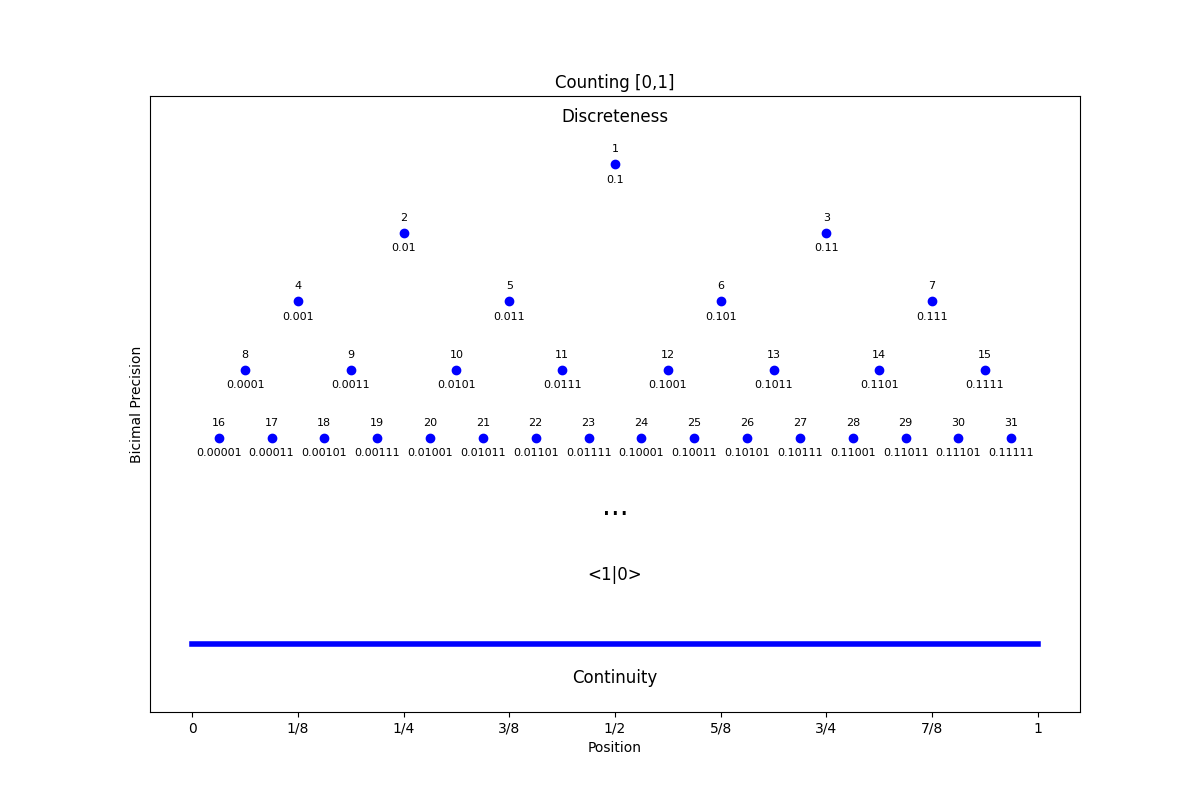
\includegraphics[width=0.95\textwidth]{continuity.png}

This sequence is particularly interesting as it itemises the [0,1] interval to ever greater precision. In the belief-based, axiomatic language of ZFC (pre-computing Cantorian mathematics) this sequence delivers a dense set, effectively showing how the real numbers between 0 and 1 would be countable were it not for the new requirement to define \qbit{} uncertainty. It is worth noting that since we can demonstrate how to count [0,1] we can use function transformations to count any continuous interval, including (-$\infty$,$\infty$) and more importantly [0,$2\pi$], provided we do not ignore \qbit{} uncertainty. This becomes important when we consider formation of the \iR{} relativistic sphere.

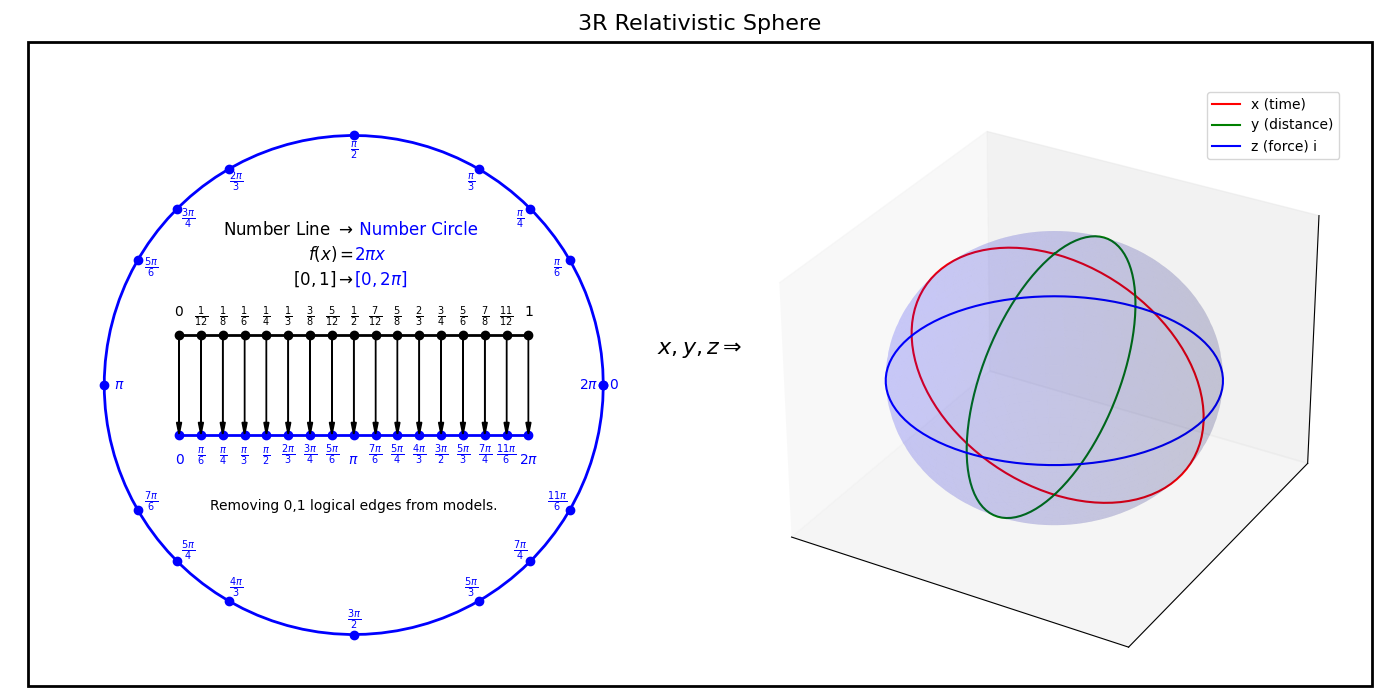
\includegraphics[width=0.95\textwidth]{3Rsphere.png}

The logical reasoning behind \qbit{} is fundamental. $\infty$ is a logic-based definition, ultimately caused by by defining \texttt{0} as \texttt{NOT 1}. The discreteness of \texttt{0} and \texttt{1} are essential features of logic but as sequences tend to $\infty$ in what logic describes as \texttt{the limit} discreteness often converges to continuity. Reality is best described as relativistic, so models are best viewed as neither continuous nor discrete but as the super-position of both. This is clearly demonstrated by quantum physics, however we can deduce the issue with far simpler examples. Logic due to its assumption of \texttt{0},\texttt{1} independence can effectively count forever. Even relatively small numbers become scientifically problematic if \qbit{} super-position is ignored. $2^{100}$ and \texttt{52!} are relatively trivial numbers mathematically but they are far from trivial in terms of scientific modelling.

Shuffle a pack of cards and the probability of any particular outcome is \texttt{1/52!}
Toss 100 coins then the probablility of any particular outcome is $2^{-100}$

These statements appear quite reasonable until you calculate just how small these numbers are. The first is approximately $1 \times 10^{-68}$ and the second is approximately $8 \times 10^{-31}$. These are not just small numbers, they are vanishingly small. Physics' Big-Bang model currently estimates the universe to be about 13.8 billion years old, approximately $3 \times 10^{19}$ seconds. Shuffle a pack of cards every second since the Big Bang and you still have only explored a miniscule fraction of the possible permutations, or toss 100 coins every second and you have explored only a tiny fraction of the possible outcomes (and a human lifetime is less than $2 \times 10^{11}$ seconds, not $3 \times 10^{19}$ seconds).

This is where we must turn to \qbit{}. It is not just a useful definition, it is an essential definition for scientific modelling. It is not reasonable to assume that reality is discrete, nor is it reasonable to assume that reality is continuous, it is reasonable to be unsure and to model the universe as the relativistic super-position of both. This is the fundamental principle of \iR{}. Clealry coin tossing and card shuffling are not simply stochastic but have singificant causal factors. We may model them as stochastic but it is a simplified model. It is a powerful model for spotting large-scale trends but a hopeless model for predicting individual outcomes. This is where \qbit{} enables logic to calculate when confidence is reasonable and conversely when more uncertainty or measurement is required. Above all else, science must always declare assumptions and quantify uncertainty.

\section*{\iR{} Dimensions}

\iR{} Dimensions is fundamental to understanding the true nature of reality. Traditionally, we often rely on binary logic—1 or 0, true or false—to make sense of the world. However, this approach is limited and does not capture the complexities and interconnectedness of real-world phenomena.

One common misunderstanding in logic and modeling is the notion that reality is constructed from a binary foundation of \texttt{0 (NOT 1)} with independent dimensions. However, this is not an accurate representation of the complexities of our world. Reality cannot be reduced to a simple binary construct; instead, it is more accurately modelled with three interlinked dimensions.

In \iR{} we introduce a third dimension which connects the other two in a relativistic manner. This third dimension is crucial as it provides a relational context that links and harmonizes the first two dimensions, offering a more comprehensive understanding of reality. This is why our brains evolved to form a three-dimensional model, allowing us to perceive and interpret the world around us more accurately.

The traditional binary logic of 1 and 0 is limited and does not account for the relative and interconnected nature of real-world phenomena. By adopting a three-dimensional approach, we acknowledge that each dimension is not independent but is instead intrinsically related to the others. This interconnectedness reflects the true nature of reality, where context and relationships play a pivotal role.

The confusion surrounding dimensions stems from an oversimplified model of logical independence. \iR{} corrects this by redefining dimensions within a relativistic model, with force acting as the dimension which links time and distance. This approach ensures a more accurate and logical model of the physical universe, addressing the limitations of classical physics. \iR{} advances our understanding of dimensions beyond the traditional \texttt{3D} model, embracing the complexities and uncertainties inherent in modelling reality. Force, as the driver of relativistic spheres, provides a unified view that elegantly ties together the concepts of time, distance, and space-time curvature.

\iR{}'s adherence to three dimensions is underpinned by rigorous logic. Strictly, dimensionality is a property of logic, but since we can only ever perceive the universe through a model, the distinction understandably becomes a little confused in most minds. Evolution perfected our animal ability to navigate and understand the environment by developing cognitive processes which model three dimensions. This evolutionary achievement is not merely a survival mechanism but a reflection of the {0,\(\qbit\),1} requirement for three relativistic dimensions. Our brain's predisposition to perceive and model dimensions evolved for a reason, optimized for interpreting the complexities surrounding us. In scientific modeling, this three-dimensional approach is not a mere preference but a logical requirement, delivering both model simplicity and detailed understanding. While logic allows the creative definition and exploration of higher dimensions, the physical and logical necessity for such dimensions is at best unnecessary and at worst highly confusing. Complex numbers, especially as used in Quantum Mechanics, underscore this point. The wave function, \(\Psi\), integral to QM, leverages complex numbers to describe the probabilistic nature of subatomic particles, and the Schrödinger equation—central to QM—demands complex numbers for its formulation and solutions. These examples highlight the sufficiency of three dimensions in modelling the fundamentals of our universe.

Evolution, traditionally perceived as a series of chance events, is more aptly described by \iR{}. Evolutionary processes are not simply random but are better modelled as \iR{}, akin to modelling quantum states in super-position. Within this context, evolutionary adaptations emerge from a complex interplay of continuous interactions and probabilistic outcomes, reflecting the {0,\(\qbit\),1} mechanisms of quantum mechanics rather than the simplicity of {0,1} binary chance. In this model, the evolutionary journey of life on Earth is seen not as a series of independent, chance occurrences but as conditional probabilities, best modelled as the super-position of causality and probability.

The alignment between evolved neural models and the logical structure found in the complex numbers of QM is profound, reinforcing the fact that our evolved sensory perception is not merely adequate but logically essential for understanding nature. \iR{} simply takes the next step to formalize this alignment, offering a comprehensive framework that integrates the cognitive, mathematical, and scientific understanding.

Applying \iR{} to a \texttt{3D} Newtonian model, we map conventional \texttt{3D} space into a \iR{} relativistic sphere, where:
\begin{itemize}
    \item the time dimension, generally modeled as the x axis, is related to velocity and direction of travel.
    \item the force dimension, generally modeled as the z or imaginary (\(i\)) axis, accounts for curving of time-distance.
    \item the distance dimension, generally modeled as the y axis, perpendicular to time and force, is the most conventional view of distance (but still part of the \iR{} curvature which ultimately delivers a relativistic sphere).
\end{itemize}

It should be noted that the concept of discrete points is replaced by relativistic spheres in \iR{} scientific models, correctly modelling uncertainty (first postulated and observed by Heisenberg). As with all modeling, however, the added complexity should be balanced against increased accuracy. Clearly, no surface on Earth is genuinely flat as the Earth is an oblate spheroid with a significant gravitational force dimension, however, for most practical purposes the Earth may be modeled as flat in a simple \texttt{3D} model with little impact on uncertainty. Model simplifications are not errors, they are required to make models practical. The key is to understand the limitations of the model in terms of \iR{} and to quantify the uncertainty.

\iR{} challenges the singularity-based, Big-Bang model of the universe, suggesting instead a continuous-relativity model, within a relativistic \iR{} sphere of time, distance, and force. This improved model explains the mystery of dark-energy and dark-matter, whilst aligning with observations, providing a coherent framework that incorporates quantum uncertainty and relativistic effects. Thus, the \iR{} time-distance-force relativistic model marks a significant departure from the Big-Bang, proposing a universe characterized by ongoing evolution and dynamic interactions best modeled with \(\qbit\) uncertainty. \iR{} offers a revolutionary perspective on the universe's structure and evolution. This model not only facilitates a deeper understanding of cosmic phenomena but also invites further exploration through theoretical and observational physics.

\section*{Beyond {0,1}: \(\qbit\)}
Logical {0,1} while foundational, often struggle when faced with the continuous and relativistic nature of reality. The introduction of \(\qbit\) represents a significant leap in logical reasoning, extending beyond {0,1} to quantify uncertainty. This extension not only supports the probabilistic models of quantum mechanics but also offers a more comprehensive tool for modeling the natural world. Much of this we do already without recognising it when we statistically fit models to experimental data.

The traditional mathematical treatment of infinity, notably in calculus, accurately embraced the concept of potential infinity. Cantor's invention of set theory in the early 20th century unfortunately made a major logical error in assuming infinite countability. It was an understandable error given it pre-dated computing and our better understanding of the defined nature of abstract number. \(\qbit\) reconciles the historically correct intuition of potential infinity with a consistent definition of number and logical \(\infty\). This is particularly important in addressing imagined paradoxes. Cantorian axioms struggle with continuous intervals such as \((0,1)\) having no smallest or largest value. The definition of \(\qbit\) within logic has no such issue, grounding the definition of \(\infty\) in a logical structure that bridges historical insights with computational rigour.

A common misconception positions computing as limited to binary operations, supposedly rendering it inadequate for tasks requiring algebraic manipulation of continuous mathematics. This view overlooks the foundational robustness of computational logic and its capacity to engage deeply with the \(\qbit\) uncertainties prevalent in scientific modelling. Computing's engagement with algebra transcends mere numerical calculations, encompassing symbolic computation or computer algebra systems (CAS) capable of performing exact algebraic manipulations. These systems, leveraging the logical rigour intrinsic to computing, can solve equations, perform differentiation and integration, and manipulate expressions symbolically. Such capabilities affirm that computing is not only suited to algebra but excels in it, addressing both discrete and continuous problems with precision.

The application of computing extends to the evaluation and testing of scientific models, where the uncertainty represented by \(\qbit\) plays a crucial role. Far from being constrained by binary limitations, modern computing methodologies—through techniques in numerical analysis, statistical modeling, and probabilistic simulations—embrace and quantify the \(\qbit\) uncertainties. This process involves sophisticated algorithms that simulate complex phenomena, providing insights into the behavior of systems under a spectrum of conditions and assumptions.

Computing's ability to navigate between discrete and continuous domains, and to apply logical operations in the service of understanding complex, uncertain systems, underscores its integral role in scientific inquiry. The binary operations of computing hardware, far from a limitation, serve as a foundation for a vast array of computational techniques that model the relativistic continuum of physical phenomena with remarkable accuracy.

The misconception that computing cannot adeptly handle algebraic manipulation or engage with the continuous and uncertain aspects of modelling physical reality is unfounded. Through the dual strengths of symbolic computation and numerical analysis, complemented by the logical framework provided by \iR{}, computing proves indispensable in both the exploration of mathematical abstractions and the empirical testing of scientific models. This dual capability not only refutes the myth of computational inadequacy but also highlights computing as a versatile, powerful tool in the advancement of knowledge, equipped to tackle the complexities of reality with rigour and precision.

\section*{Numbers}

In the realm of logic, the representation and understanding of numbers is crucial. Logic defines numbers exactly, with potentially infinite precision. Scientific inquiry in contrast accepts inherent (and logically unavoidable) measurement uncertainty. Computing straddles these realms, supporting either and both. In all cases it is essential to recognise that numbers are not real. Numbers are defined by logic, created to model and understand the universe. They are an extremely sophisticated and powerful form of words.

Constants like \(\pi\) and \(\sqrt{2}\) show how logic defines complete precision, using endless digits. The mathematical constant \(\pi\), renowned for its infinite, non-repeating representation is a key example. Algorithms exist which enable the calculation of any digit of \(\pi\), exemplified by the Bailey–Borwein–Plouffe (BBP) formula.
\[ \pi = \sum_{k=0}^{\infty} \left( \frac{1}{16^k} \left( \frac{4}{8k + 1} - \frac{2}{8k + 4} - \frac{1}{8k + 5} - \frac{1}{8k + 6} \right) \right) \]
This algorithmic approach resonates with the essence of \(\qbit\), as it showcases the ability to navigate the potentially infinite precision of \(\pi\) with a methodological clarity and efficiency. Recognising \(\qbit\) in the expansion of \(\pi\), highlights the structured yet boundless nature of mathematical constants. \(\pi\)'s hexadecimal digits, determinable through the BBP formula, demonstrates the structured approach to \(\infty\) that \(\qbit\) enables—where each digit represents a finite point of clarity within a potentially infinite expanse.

Incorporating \(\qbit\) into our discussion of \(\pi\) and similar constants not only enriches our mathematical discourse but also highlights the practical utility of \(\qbit\) in navigating the complexities of \(\infty\) with precision and rigour. This methodology fosters a deeper appreciation for the elegance of mathematical constants and the innovative algorithms that allow us to explore them, bridging historical intuition with computational rigour.

Contrastingly, science operates with uncertainty, dealing with precision limited by both theoretical and practical observational accuracy. Scientific numbers, such as measurements and scientific constants, carry quantifiable uncertainty. This uncertainty may be represented like \(11.01001\qbit\), where \(\qbit\) marks the threshold beyond which certainty fades into probabilistic indeterminacy.

Computing addresses the need for numerical precision in a manner that surpasses the demands of scientific accuracy, supporting algebraic precision when required. Floating-point numbers, the default type in computing, offer a balance, supporting a vast range of values significantly beyond logically provable limits in scientific accuracy (such as Heisenberg uncertainty). Computing's ability to manipulate logical values perfectly whilst tracking and calculating the uncertainty of scientific values makes it invaluable in modelling reality.

Within this spectrum, programmers and AI systems face the crucial task of selecting the appropriate numerical representation for their specific needs:
- Algebraic coding techniques are employed for tasks demanding the highest degree of precision, aligning with the exacting standards of mathematical logic and proof.
- General-purpose floating-point representations suffice for the vast majority of scientific and practical applications, where the infinitesimal details lost to finite precision are of negligible consequence.

The use of numbers across different disciplines reveals a varied landscape of precision, uncertainty, and practicality. From the infinite precision of logical constants, through the uncertain measurements of science, \iR{} offers a diverse set of tools and methods, harnessing the capabilities of computing to model and understand reality to quantifiable levels of certainty.

\section*{Conclusion}

The journey of understanding and applying \iR{} is not solely about advancing technology or achieving personal accolades. It is about collectively harnessing our intellectual and ethical capabilities to reshape politics, economics, law, and society. The focus must shift from individual fame and greed to enhancing the quality of life and protecting our ecosystem.

By embracing the principles of \iR{} scientific modelling, we can build systems that reflect the intricate realities of our world, fostering informed and ethical decisions. These decisions, driven by a clear understanding of continuous-relativity and logical rigour, will guide us towards a society where human and ecological well-being is prioritised over short-term gains.

Together, we can create a future where logical integrity and ethical considerations are at the heart of our collective choices. This future envisions a society that is not only sustainable but also equitable and enjoyable, ensuring that the human species thrives harmoniously within our ecosystem.

The task ahead is significant, but it is also a unique opportunity. This transformation is not just possible—it is essential for the survival and flourishing of our planet and all its inhabitants.

It is widely acknowledged that our current political and economic systems are disastrous. However, what is less understood is that these systems can be fixed. Central to this transformation is the need to fix AI. Currently, AI is being used not to teach logic and help society, but to accelerate the illogical, rapid destruction of the environment driven by individual greed.

My history gives me a unique perspective and skill set, enabling me to see solutions that others may not. While it may take a generation for everyone to fully grasp the concepts explained in this paper, the best way to learn is by doing. Therefore, I will be building systems that allow people to see for themselves what is possible.

By demonstrating the potential of these systems, we can inspire a shift towards a more logical and ethical approach, ultimately creating a sustainable and harmonious future. It is through our combined efforts and commitment to these principles that we can achieve a balanced existence on Earth, ensuring a better future for generations to come.

\section*{Physics - \iR{} Work in Progress}

This is not my priority, but it is an interesting hobby. My primary focus is to develop a new, inherently logical, \iR{} AI. My background is in Computer Science and Mathematics, not Physics, but I have always loved mechanics, and have increasing come to recognise the importance of statistics in logical modelling of scientific, discrete-continuous, super-position. The sections below are largely the work of AI which has been trained on my \iR{} text. I have made some minor edits to improve the flow and clarity, but the content is largely the work of AI. As a computer programmer with over 40 years experience I rarely now write code without AI at least building the first version. My AI coding buddy is a language not a logic model, so makes both logical and understanding errors, but its underlying hardware is billions of times faster and more reliable than my brain. Once developed \iR{} AI can be guided to review and correct the content below. For now any human brains are most welcome to give it a shot.

\iR{} with its focus on modelling the interconnectedness of reality, offers a comprehensive understanding of atomic systems like the hydrogen atom and cosmological phenomena. By integrating \iR{} with quantum mechanics and cosmology, we provide a unified framework that bridges the microscale and macroscale models of the universe. This approach not only demystifies the mathematics behind quantum and cosmic phenomena but also aligns with the 3R model's emphasis on a holistic understanding of reality. The goal is to help physicists understand and correct existing models, paving the way for advancements in both theoretical and applied physics.

\subsection*{The \(\iR\) Hydrogen Atom}

In the journey to reconcile quantum mechanics with the 3R model, an initial focus is on the hydrogen atom. Traditionally, the Hartree model is used in quantum chemistry to approximate electron distributions. The Hartree model approaches the multi-electron problem by assuming that each electron moves independently in the average field created by the nucleus and the other electrons. This simplification leads to a set of self-consistent field equations:

\[
    \left[ -\frac{\hbar^2}{2m}\nabla^2 - \frac{Ze^2}{4\pi\epsilon_0 r} + V_{\text{eff}}(r) \right] \psi(r) = E\psi(r),
\]

where \(\psi(r)\) is the wavefunction of the electron, \(E\) is its energy, and \(V_{\text{eff}}(r)\) is the effective potential experienced by the electron.

Within the 3R framework, the nucleus (in the case of hydrogen, a single proton) forms the foundational time-force-distance standing wave. This central wave influences the electron's wavefunction through a complex interaction that includes the principles of the 3R model. By redefining the effective potential in the Hartree equation to include a 3R influence factor, we obtain:

\[
    V_{\text{3R-eff}}(r) = V_{\text{eff}}(r) + \Delta V_{\text{3R}}(r),
\]

where \(\Delta V_{\text{3R}}(r)\) represents the modification to the potential due to the 3R model. This term encapsulates the effect of the nucleus' standing wave on the electron, integrating traditional physics with the broader principles of the 3R framework.

Quantum mechanics introduces inherent uncertainty in the behavior of particles, notably electrons in atoms. This model uncertainty is quantified by \qbit{} and the Heisenberg Uncertainty Principle, which states that the position and momentum of a particle cannot both be precisely determined simultaneously. In the context of the hydrogen atom, this principle influences the electron's energy states and its probabilistic distribution around the nucleus. The electron in a hydrogen atom exists in discrete energy states, or orbitals, which are solutions to the Schrödinger equation:

\[
    -\frac{\hbar^2}{2m}\nabla^2 \psi(\mathbf{r}) + V(\mathbf{r})\psi(\mathbf{r}) = E\psi(\mathbf{r}),
\]

where \(\psi(\mathbf{r})\) is the wavefunction, \(V(\mathbf{r})\) is the potential energy function, and \(E\) represents the energy levels.

In Hartree atomic units, where \(\hbar = m = e = 4\pi\epsilon_0 = 1\), the Schrödinger equation simplifies to:

\[
    -\frac{1}{2}\nabla^2 \psi(\mathbf{r}) - \frac{1}{r}\psi(\mathbf{r}) = E\psi(\mathbf{r}),
\]

making the complex quantum mechanical behaviors more accessible. The \iR{} model emphasizes modelling the electron as existing in a state of quantum super-position described by its wavefunction. The uncertainty in the electron's position and energy is fundamental, influencing the atom's chemical and physical properties.

A key dimensionless quantity derived from quantum electrodynamics and the Hartree model is the fine structure constant (\(\alpha\)), characterizing the strength of electromagnetic interactions:

\[
    \alpha = \frac{e^2}{4\pi \epsilon_0 \hbar c}.
\]

In Hartree units, this simplifies, highlighting its fundamental role in mediating interactions within the hydrogen atom. The time-distance-force sphere can be described using the wavefunction \(\psi(r, t)\) and a modified Schrödinger equation that includes a force term:

\[
    i \frac{\partial \psi}{\partial t} = \left( -\frac{1}{2} \nabla^2 + V(r) + iF \right) \psi,
\]

where \(V(r) = -\frac{1}{r}\) and \(F = -i \frac{1}{r^2}\). By introducing this complex force term, the equation reflects the interdependent nature of time, distance, and force, embodying the principles of the 3R framework.

\subsection*{The \(\iR\) Universe}

Extending the \(\iR\) model to cosmology, we reinterpret the universe as a \(\iR\) sphere, conceptualizing it as a continuous convection cycle where light energy condenses into hydrogen, stars, matter and eventually into black holes, before being re-radiated. This perspective challenges the traditional Big Bang theory by removing the concepts of a distinct beginning and end, emphasising instead a perpetual cycle of energy transformation and matter condensation.

In this model, light energy condenses into matter through processes similar to those observed in stellar formation. Over time, matter aggregates into larger structures, eventually forming black holes. Black holes, in this framework, are not endpoints but part of a dynamic cycle. The intense gravitational forces within black holes compress matter and energy, which can be re-radiated as high-energy particles and radiation, observed as jets in side-on views of black holes.

The edge of the universe is a horizon not an edge, where the rotating light energy from distant objects is indistiguishable from background radiation. Background radiation is not a remnant of some Big Bang but simply the light energy from distant objects which has been red-shifted to the point of being indistinguishable from the background radiation. The universe is not expanding, it is rotating. The universe is not a 3D sphere, it is a \iR{} sphere.

This continuous cycle aligns with \iR{} principles by emphasising the interdependence and transformation of energy and matter across different scales of the universe. By viewing the universe as a \iR{} sphere, we gain insights into the fundamental processes driving cosmic evolution and the interplay between light, matter, and black holes.

\end{document}
